\chapter{Implementación}
\label{implementacion}

Hasta ahora, con todas las piezas de información que hemos generado acerca del desarrollo, hemos podido, en efecto, discernir entre tres grandes grupos de tareas: la gestión, el calendario y el panel de control. Así pues, estableceremos la separación del desarrollo en estos tres grandes bloques de trabajo, con la previa especificación de las herramientas a utilizar y del trabajo anterior al comienzo del proceso de programación, propiamente dicho, que implican la puesta a punto de la base de datos y del servidor para probar y desarrollar nuestra aplicación.

\section{Herramientas para el desarrollo de twinX}

Para llevar a cabo la programación de este sitio web, aunque utilicemos herramientas más sofisticadas, éstas están basadas en los clásicos lenguajes web: \textbf{HTML} (\textit{HyperText Markup Language}) \cite{html} para la estructuración de la web y la identificación de los distintos elementos, \textbf{CSS} \cite{css} (\textit{Cascading Style Sheets}) para aplicar estilo a la vista (posicionamiento, colores, visibilidad, etc.) y JavaScript \cite{javascript}, para implementar funciones más complejas a cada componente de la web. Para el manejo de estos dos últimos, contaremos con la ayuda de dos librerías con un gran potencial. Para el estilo, usaremos \textbf{Bootstrap} \cite{bootstrap} en su cuarta versión y para JavaScript utilizaremos \textbf{jQuery} \cite{jquery}. Nos permitirán ahorrar mucho tiempo, ya que en ambos casos podemos hacer uso de funciones o palabras clave que evitarán el tener que escribir numerosas líneas de código en cada uno de los lenguajes a los que complementan.

Como ya hemos mencionado en varias ocasiones, el desarrollo va a ser llevado a cabo con la ayuda de Yii2 Framework. En su segunda versión, este framework hace uso del lenguaje de programación PHP para orquestar múltiples tareas que resultan algo engorrosas de llevar a cabo sin su ayuda, como son, por ejemplo, las operaciones con la base de datos o la generación de código del que partir para dar forma a la vista, modelo o controlador de alguna de las secciones de twinX \cite{yii}.

Entre sus características, destacamos el generador de código Gii (figura \ref{fig:gii}), que puede automatizar la creación, por ejemplo, de la clase de un modelo, o incluso de una tabla CRUD al completo (esto es, su vista y su controlador). Tan solo tenemos que indicar cuál es la tabla de la base de datos sobre la que queremos generar los fragmentos de código, y atendiendo a las restricciones creadas en la misma, se puede obtener fácilmente una clase instanciable para recuperar o guardar información en su tabla. Del mismo modo, al crear una tabla CRUD, tendríamos directamente en nuestro sitio web una interfaz donde pueden verse los registros almacenados en la base de datos, con la posibilidad de crear nuevos, eliminarlos o incluso filtrarlos y editarlos. No cabe duda del potencial de esta característica, la cual nos permitirá ahorrar mucho tiempo y seguridad a la hora de desarrollar y de depositar la confianza en código automáticamente generado y sin errores.

\begin{figure}
	\centering
	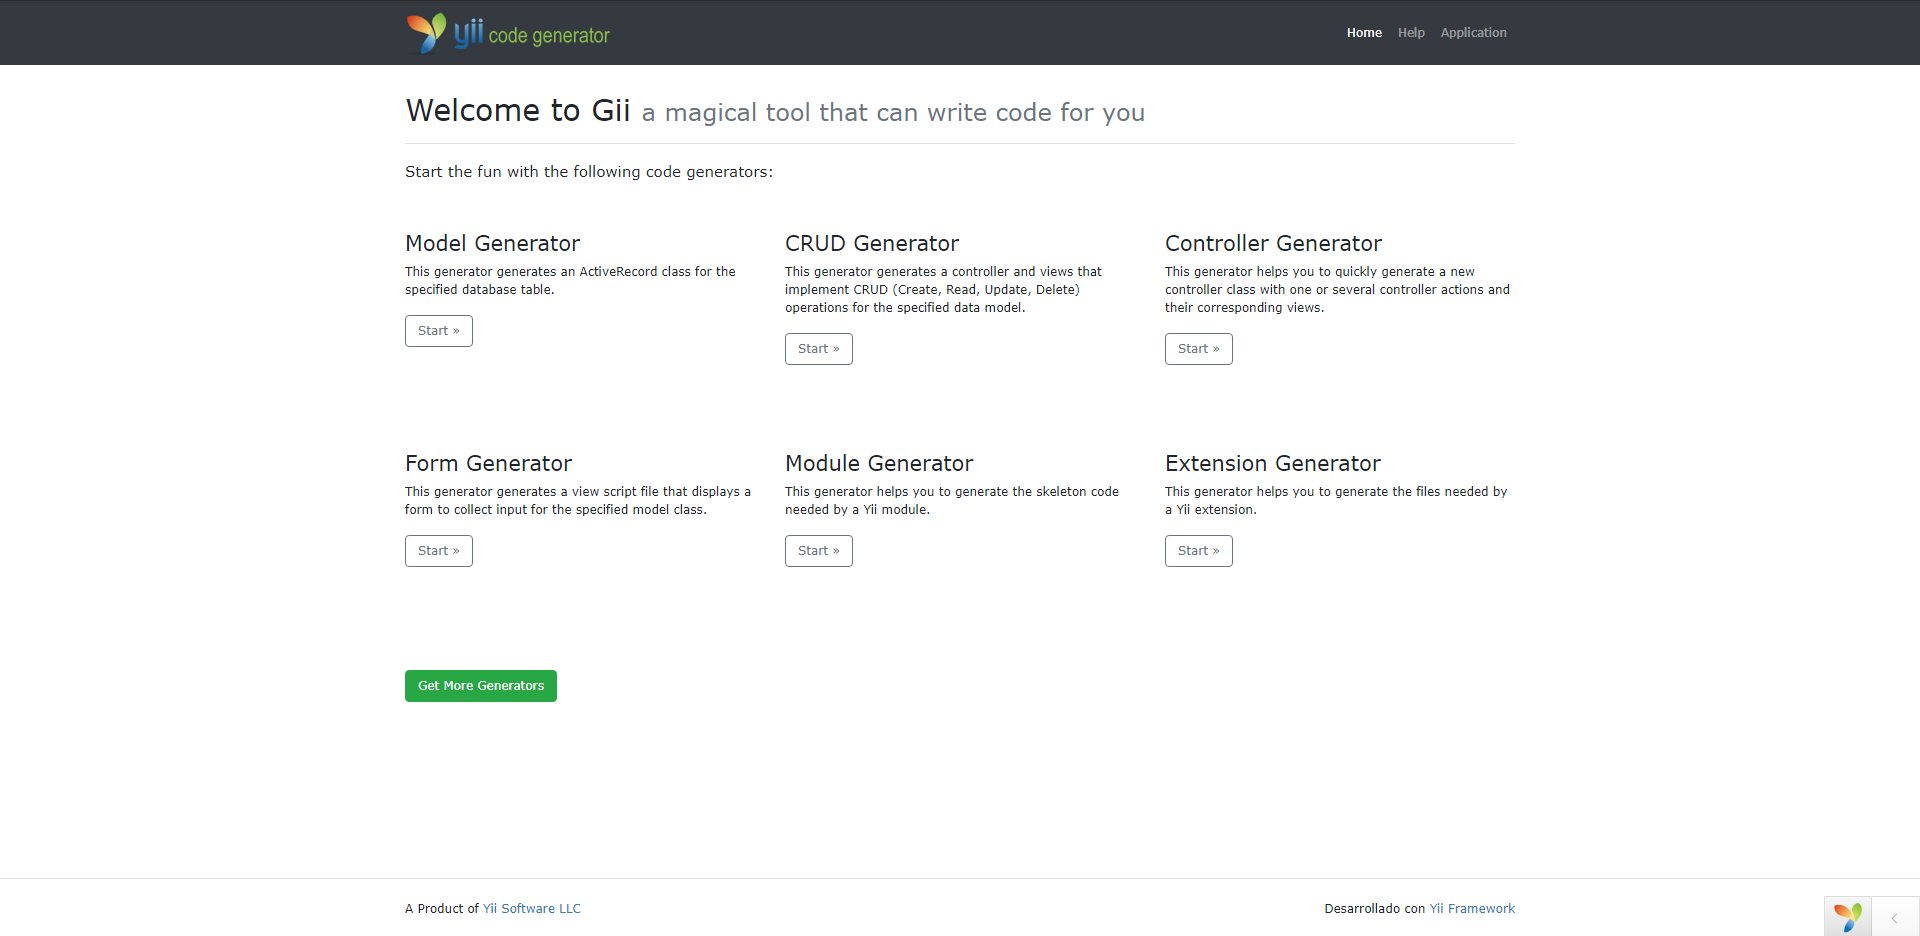
\includegraphics[width=\textwidth]{gii}
	\caption[Portal de Gii]{Portal de Gii desde donde podemos seleccionar un tipo de elemento a crear para que genere su código fuente}
	\label{fig:gii}
\end{figure}


Para comenzar a usar Yii, lo primero que tenemos que hacer es hacernos con el gestor de dependencias de PHP \textbf{Composer} \cite{composer} y descargarnos el esqueleto de un proyecto en Yii2 avanzado \cite{yii2advanced}. Para ello, basta con escribir:

\par\noindent\rule{\textwidth}{0.4pt}
\texttt{composer create-project --prefer-dist yiisoft/yii2-app-advanced twinX}
\smallskip

Y con ello ya tendríamos la carpeta con nuestro proyecto. Concretamente este directorio es el que tenemos que servir y al que nos conectaremos para visualizar nuestra web. También tenemos que seguir los pasos en el repositorio de GitHub de yiisoft para aplicar los ajustes necesarios derivados del renombramiento y redireccionamiento de URLs en el servidor. También tendremos que instalar algunas dependencias haciendo uso de la orden \texttt{composer install} y de iniciar el entorno de desarrollo con el archivo \texttt{ini} de PHP que incluye el repositorio que hemos clonado.

A continuación, procederemos con la instalación de la pila software \textbf{XAMPP} (Apache, MariaDB, PHP y Perl). En Windows, es una instalación sencilla a través de una interfaz de usuario, por lo que no requiere un gran tiempo. Es importante que, una vez instalado, situemos la carpeta del proyecto dentro del directorio \texttt{htdocs}, en la raíz de la carpeta de instalación de xampp. Se recomienda instalar en el directorio C:\ en Windows. En nuestro caso, hemos hecho los ajustes necesarios para poder situar esta carpeta en otro directorio desde donde se trabaja con el repositorio GitHub del proyecto, para que de forma más cómoda podamos salvaguardar el progreso del desarrollo de forma periódica sin tener que copiar archivos de un directorio que esté fuera del repositorio.

Esta pila contiene también la apliación \textbf{phpMyAdmin}, que ha sido también una gran ayuda para poder visualizar las tablas en base de datos, acceder a registros concretos o ejecutar código SQL desde una interfaz gráfica. Frente a una terminal desde donde manejar la base de datos, presenta una menor tasa de errores al introducir órdenes, pues la información puede verse a golpe de click y con una presentación más vistosa.

Sobre GitHub, al comienzo de la redacción de esta memoria se creó el repositorio \cite{repogit} donde, mediante la creación de ramas, hemos ido guardando en distintos commits las versiones del proyecto. Una vez creada una pieza de valor, se hacía una mezcla (\textit{merge}) a la rama \texttt{master}, de modo que cada rama se creaba con un fin, para añadir una nueva funcionalidad, sin depender del funcionamiento de las demás, para que poco a poco se puedan ir integrando las funcionalidades en su totalidad.

Finalmente, otro de los protagonistas del desarollo es el IDE (\textit{integrated development environment}) con que se ha programado twinX. En este caso, haciendo uso de su licencia educativa, se ha usado PhpStorm \cite{phpstorm}. Ha sido esencial, pues hemos descartado otras herramientas como Visual Studio Code ya que no tienen tan buen integración con PHP y Yii en sí como tiene este IDE. Destacan también características como su guardado automático inteligente, su potente búsqueda de archivos y sus cómodos atajos de teclado. Todo ello han hecho el proceso de desarrollo muy cómodo y liviano.


\section{Creación de la base de datos}

Tal y como hemos indicado en la sección \ref{sec:modelobd}, para crear el esquema del modelo de la base de datos, hemos usado la herramienta dbdiagram.io \cite{dbdiagram}. Ésta tiene mucho potencial, pues no es un simple creador de diagramas. Su principal característica es la confección de la parte gráfica mediante una especie de lenguaje creado por los mismos creadores, DBML \cite{dbml}. Con él, se pueden especificar tablas, atributos, estructuras de enumeración y características de los atributos, como claves externas, primarias, cardinalidades y la posibilidad de que un atributo pueda o no ser nulo. Gracias a ello, se ha podido mejorar progresivamente el modelo de la base de datos, pues un cambio en el código implica una variación en la visualización de las tablas, bien sea con algún atributo de más o alguna nueva relación entre tablas.

No solo es posible ver con mayor claridad las características del modelo en el código en DBML, sino que también tiene la gran posibilidad de exportarlo a otro lenguaje como es SQL. De este modo, con tan solo unos clicks, se obtienen las órdenes que posteriormente phpMyAdmin entenderá y podrá crear todas las tablas por nosotros, con todas las restricciones establecidas y ahorrando, así, mucho tiempo.

En la práctica, el código que tenemos en DBML para generar el modelo de la figura \ref{fig:modeloBD} es:

\newpage
\begin{lstlisting}
	// ENTIDADES BASICAS
	
	Table centro as CEN {
		id int [pk, increment]
		nombre varchar [not null, unique]
	}
	
	Table curso as CURSO {
		id int [pk, increment]
		curso varchar(4) [not null]
	}
	
	Table mail_predef as MAIL {
		id int [pk, increment]
		titulo varchar [not null, unique]
		asunto varchar [not null]
		cuerpo text [not null]
	}
	
	Table titulacion as TIT {
		id int [pk]
		nombre varchar [not null, unique]
		id_centro int [not null]
	}
	
	Ref: TIT.id_centro > CEN.id
	
	Table asignatura as ASIG {
		id int [pk]
		id_tit int [not null]
		nombre varchar [not null]
		ects int [not null]
		cuatrimestre cuatrimestre [not null]
		tipo tipo_asignatura [not null]
	}
	
	Ref: ASIG.id_tit > TIT.id
	
	Table asignatura_ext as EXT_ASIG {
		id int [pk]
		id_conv int [not null] 
		nombre varchar [not null]
		ects int [not null]
		id_curso int [ref: > CURSO.id, not null] 
		cuatrimestre cuatrimestre [not null]
	}
	
	Ref: EXT_ASIG.id_conv > CON.id
	
	Table pais as P {
		iso varchar [pk]
		nombre varchar [not null]
	}
	
	Table universidad as UNI {
		cod_uni varchar [not null]
		cod_pais varchar [not null]
		nombre varchar [not null]
		direccion varchar 
		web varchar
		email varchar
		
		Indexes {
			(cod_pais, cod_uni) [pk]
		}
	}
	
	Ref: UNI.cod_pais > P.iso
	
	Table area as AR {
		cod_isced varchar [pk]
		nombre_isced varchar [not null]
		nombre_area varchar 
		
	}
	
	// USUARIOS Y TIPOS
	
	Table user as U {
		id int [pk, increment]
		username varchar
		nombre varchar
		tipo tipo_usuario
		password varchar
		email varchar
		telefono varchar
		genero genero
	}
	
	Table estudiante as EST{
		id_usuario int [not null]
		dni varchar [not null, unique] // PUEDE SER NIE
		id_convenio int [not null]
		id_titulacion int [not null]
		telefono2 int 
		email_go_ugr varchar 
		f_nacimiento datetime [not null]
		tipo_estudiante tipo_estudiante [not null]
		cesion_datos boolean 
		nota_expediente double 
		beca_mec boolean
	}
	
	Ref: EST.id_titulacion > TIT.id
	Ref: U.id - EST.id_usuario
	Ref: EST.id_convenio > CON.id
	
	
	// CONVENIOS Y ACUERDOS
	
	Table competencia_ling as CL {
		id int [pk, increment]
		lengua varchar [not null]
		nivel nivel_idioma [not null]
	}
	
	Table rel_cl_est {
		id int [pk, increment]
		id_cl int [ref: > CL.id, not null]
		id_est int [ref: > EST.id_usuario, not null]
	}
	
	Table req_ling_conv {
		id int [pk, increment]
		id_comp int [ref: > CL.id, not null]
		id_conv int [ref: > CON.id, not null]
	}
	
	Table convenio as CON {
		id int [pk, increment]
		cod_area varchar [not null]
		cod_uni varchar [not null]
		cod_pais varchar [not null]
		id_admon_out int
		
		id_curso_creacion int [ref: > CURSO.id, not null]
		creado_por int [not null]
		
		num_becas_in int [not null]
		num_becas_out int [not null]
		
		meses_in int [not null]
		meses_out int [not null]
		
		anno_inicio int [not null]
		anno_fin int [not null]
		
		req_titulacion varchar
		req_curso varchar
		
		nominacion_online boolean 
		link_nom_online varchar 
		info_nom_online text
		
		link_documentacion varchar
		
		movilidad_pdi boolean 
		movilidad_pas boolean 
		
		tipo_movilidad tipo_movilidad [not null]
		
		user_online varchar
		password_online varchar
		fecha_online datetime
		
		info_tor text 
		
		observ_discapacidad text
		observ_req_ling text 
		
		begin_nom_1s datetime
		end_nom_1s datetime
		begin_nom_2s datetime
		end_nom_2s datetime
		begin_app_1s datetime
		end_app_1s datetime
		begin_app_2s datetime
		end_app_2s datetime
		begin_mov_1s datetime
		end_mov_1s datetime
		begin_mov_2s datetime
		end_mov_2s datetime
		
		memo_grading text
		memo_visado text
		memo_seguro text
		memo_alojamiento text
		
		nombre_coord varchar
		cargo_coord varchar
		email_coord varchar
		tlf_coord varchar
		address_coord varchar [note:"Por defecto igual que la de la universidad"]
		web_inf_acad varchar
		
		nombre_admon_in varchar
		cargo_admon_in varchar
		mail_admon_in varchar
		nombre_resp_acad_in varchar
		cargo_resp_acad_in varchar
		
		nombre_admon_out varchar
		cargo_admon_out varchar
		mail_admon_out varchar
		nombre_resp_acad_out varchar
		cargo_resp_acad_out varchar
		mail_resp_acad_out varchar
		
	}
	
	Ref: P.iso < CON.cod_pais
	Ref: CON.creado_por > U.id
	Ref: CON.cod_area > AR.cod_isced
	Ref: CON.(cod_pais, cod_uni) > UNI.(cod_pais, cod_uni)
	
	
	Table acuerdo_estudios as AE {
		id int [pk, increment]
		id_estudiante int [not null]
		id_tutor int [not null]
		
		timestamp_creacion datetime [not null]
		periodo cuatrimestre [not null]
		fase int [not null]
		id_curso int [ref: > CURSO.id, not null]
		necesidades text
		begin_movilidad date // comienzo individual del estudiante
		end_movilidad date // fin individual del estudiante
		timestamp_nominacion datetime 
		timestamp_registro datetime [not null]
		link_documentacion varchar
		n_solicitud_RRII int
		convocatoria convocatoria [not null]
	}
	
	Ref: AE.id_estudiante > EST.id_usuario
	Ref: AE.id_tutor > U.id
	
	Table ae_asigloc_asigext {
		id_ae int
		asig_loc int [ref: > ASIG.id]
		asig_ext int [ref: > EXT_ASIG.id]
		
		Indexes {
			(id_ae, asig_loc, asig_ext) [pk]
		}
	}
	
	Table renuncia as REN{
		id int [pk, increment]
		id_ae int  [not null, ref: - AE.id]
		descripcion text [not null]
		timestamp datetime [not null]
	}
	
	// EXPEDIENTES, TIPOS DE EXPDIENTE Y FASES
	
	Table expediente as EXP{
		id int [pk, increment]
		id_ae int [not null]
		id_tipo_exp int [not null]
	}
	
	Ref: EXP.id_ae > AE.id
	Ref: EXP.id_tipo_exp > TIPO_EXP.id
	
	Table tipo_expediente as TIPO_EXP {
		id int [pk, increment]
		descripcion varchar [not null]
		tipo_estudiante tipo_estudiante [not null]
	}
	
	Table fase_expediente as FAS_EXP {
		id int [pk, increment]
		id_tipo_exp int [not null]
		descripcion varchar [not null]
		fase_final boolean [default: 0]
	}
	
	Ref: FAS_EXP.id_tipo_exp > TIPO_EXP.id
	
	Table envio_mail_fase {
		id int [pk, increment]
		id_mail int [ref: > MAIL.id, not null]
		id_fase int [ref: > FAS_EXP.id, not null]
		cargo cargo [not null]
	}
	
	Table hist_envio_mail_fase {
		id int [pk, increment]
		id_mail int [ref: > MAIL.id, not null]
		id_fase int [ref: > FAS_EXP.id, not null]
		id_exp int [ref: > EXP.id, not null]
		email varchar [not null]
	}
	
	Table hist_envio_mail_fase_mod { // Mail modificado
		id int [pk, increment]
		asunto varchar
		cuerpo text [not null]
		id_fase int [ref: > FAS_EXP.id, not null]
		id_exp int [ref: > EXP.id, not null]
		email varchar [not null]
	}
	
	Table rel_exp_fase as REL_EF {
		id int [pk]
		id_exp int [not null]
		id_fase int [not null]
		id_gestor int [not null]
		procesado boolean 
		timestamp datetime [not null]
		info varchar
	}
	
	Ref: REL_EF.id_exp - EXP.id
	Ref: REL_EF.id_fase - FAS_EXP.id
	Ref: REL_EF.id_gestor - U.id
	
	Table rel_exp_fav_gestor { 
		id int [pk, increment]
		id_exp int [ref: > EXP.id]
		id_gestor int [ref: > U.id]
		//tipo_usuario == GESTOR
	}
	
	// CALENDARIO
	
	Table evento as EV {
		id int [pk, increment]
		id_creador int [not null]
		titulo varchar [not null]
		descripcion text
		estado estado_evento_tarea [not null]
		prioridad prioridad [not null, default: 'MEDIA']
	}
	
	Ref: EV.id_creador - U.id //tipo == GESTOR
	
	Table tarea as TASK {
		id int [pk, increment]
		descripcion text [not null]
		estado estado_evento_tarea [not null, default: 'PENDIENTE']
	}
	
	Table deadline_aviso as DLA { 
		id int [pk, increment]
		fecha datetime [not null]
		id_responsable int [not null]
		id_evento int  [not null]
		id_tarea int [not null]
	}
	
	Ref: DLA.id_responsable > U.id // tipo == GESTOR
	Ref: DLA.id_evento > EV.id
	Ref: DLA.id_tarea > TASK.id
	
	Table recordatorio {
		id int [pk, increment]
		timestamp datetime [not null]
		id_usuario int [ref: > U.id, not null]
		deadline datetime [not null]
		titulo varchar [not null]
		descripcion text
		completado boolean
	}
	
	
	// MENSAJES	
	Table mensaje as MSG{
		id int [pk, increment]
		timestamp datetime [not null]
		id_emisor int [not null]
		id_receptor int [not null]
		leido boolean
		etiqueta etiqueta_msg [not null]
		asunto varchar 
		cuerpo text [not null]
		
	}
	
	Ref: MSG.id_emisor > U.id
	Ref: MSG.id_receptor > U.id
	
	Enum tipo_asignatura {
		TRONCAL
		OBLIGATORIA
		OPTATIVA
	}
	
	Enum cargo {
		COORDINADOR
		ADMON_IN
		ADMON_OUT
		RESP_ADMON_OUT
	}
	
	Enum nivel_idioma {
		B1
		B2
		C1
		C2
	}
	
	
	Enum etiqueta_msg {
		IMPORTANTE
		ELIMINADO
	}
	
	Enum estado_evento_tarea {
		PENDIENTE
		EN_PROCESO
		TERMINADO
	}
	
	Enum prioridad {
		ALTA
		MEDIA
		BAJA
	}
	
	Enum estado_ae {
		REVISION
		DENEGADO
		ACEPTADO
		VIGENTE
	}
	
	Enum convocatoria {
		PRIMERA
		SEGUNDA
		EXTRAORDINARIA
	}
	
	Enum tipo_movilidad {
		ERASMUS
		ARQUS
		ERASMUS_DI
		ERASMUS_PARTNER
		INTERCAMBIO
		LIBRE_MOVILIDAD
	}
	
	Enum tipo_usuario {
		SUPERUSUARIO
		GESTOR
		ESTUDIANTE
		TUTOR
	}
	
	Enum genero {
		F
		M
		O
	}
	
	Enum tipo_estudiante {
		INCOMING
		OUTGOING
	}
	
	Enum cuatrimestre {
		PRIMERO
		SEGUNDO
		C_COMPLETO
	}
	
\end{lstlisting}

Y como resultado, podemos traducir todo ello a código SQL, quedando de la siguiente manera:
\lstset{breaklines=true}
\begin{lstlisting}[language=sql]
	
	CREATE TABLE `centro` (
	`id` int PRIMARY KEY AUTO_INCREMENT,
	`nombre` varchar(255) UNIQUE NOT NULL
	);
	
	CREATE TABLE `curso` (
	`id` int PRIMARY KEY AUTO_INCREMENT,
	`curso` varchar(4) NOT NULL
	);
	
	CREATE TABLE `mail_predef` (
	`id` int PRIMARY KEY AUTO_INCREMENT,
	`titulo` varchar(255) UNIQUE NOT NULL,
	`asunto` varchar(255) NOT NULL,
	`cuerpo` text NOT NULL
	);
	
	CREATE TABLE `titulacion` (
	`id` int PRIMARY KEY,
	`nombre` varchar(255) UNIQUE NOT NULL,
	`id_centro` int NOT NULL
	);
	
	CREATE TABLE `asignatura` (
	`id` int PRIMARY KEY,
	`id_tit` int NOT NULL,
	`nombre` varchar(255) NOT NULL,
	`ects` int NOT NULL,
	`cuatrimestre` ENUM ('PRIMERO', 'SEGUNDO', 'C_COMPLETO') NOT NULL,
	`tipo` ENUM ('TRONCAL', 'OBLIGATORIA', 'OPTATIVA') NOT NULL
	);
	
	CREATE TABLE `asignatura_ext` (
	`id` int PRIMARY KEY,
	`id_conv` int NOT NULL,
	`nombre` varchar(255) NOT NULL,
	`ects` int NOT NULL,
	`id_curso` int NOT NULL,
	`cuatrimestre` ENUM ('PRIMERO', 'SEGUNDO', 'C_COMPLETO') NOT NULL
	);
	
	CREATE TABLE `pais` (
	`iso` varchar(255) PRIMARY KEY,
	`nombre` varchar(255) NOT NULL
	);
	
	CREATE TABLE `universidad` (
	`cod_uni` varchar(255) NOT NULL,
	`cod_pais` varchar(255) NOT NULL,
	`nombre` varchar(255) NOT NULL,
	`direccion` varchar(255),
	`web` varchar(255),
	`email` varchar(255),
	PRIMARY KEY (`cod_pais`, `cod_uni`)
	);
	
	CREATE TABLE `area` (
	`cod_isced` varchar(255) PRIMARY KEY,
	`nombre_isced` varchar(255) NOT NULL,
	`nombre_area` varchar(255)
	);
	
	CREATE TABLE `user` (
	`id` int PRIMARY KEY AUTO_INCREMENT,
	`username` varchar(255),
	`nombre` varchar(255),
	`tipo` ENUM ('SUPERUSUARIO', 'GESTOR', 'ESTUDIANTE', 'TUTOR'),
	`password` varchar(255),
	`email` varchar(255),
	`telefono` varchar(255),
	`genero` ENUM ('F', 'M', 'O')
	);
	
	CREATE TABLE `estudiante` (
	`id_usuario` int NOT NULL,
	`dni` varchar(255) UNIQUE NOT NULL,
	`id_convenio` int NOT NULL,
	`id_titulacion` int NOT NULL,
	`telefono2` int,
	`email_go_ugr` varchar(255),
	`f_nacimiento` datetime NOT NULL,
	`tipo_estudiante` ENUM ('INCOMING', 'OUTGOING') NOT NULL,
	`cesion_datos` boolean,
	`nota_expediente` double,
	`beca_mec` boolean
	);
	
	CREATE TABLE `competencia_ling` (
	`id` int PRIMARY KEY AUTO_INCREMENT,
	`lengua` varchar(255) NOT NULL,
	`nivel` ENUM ('B1', 'B2', 'C1', 'C2') NOT NULL
	);
	
	CREATE TABLE `rel_cl_est` (
	`id` int PRIMARY KEY AUTO_INCREMENT,
	`id_cl` int NOT NULL,
	`id_est` int NOT NULL
	);
	
	CREATE TABLE `req_ling_conv` (
	`id` int PRIMARY KEY AUTO_INCREMENT,
	`id_comp` int NOT NULL,
	`id_conv` int NOT NULL
	);
	
	CREATE TABLE `convenio` (
	`id` int PRIMARY KEY AUTO_INCREMENT,
	`cod_area` varchar(255) NOT NULL,
	`cod_uni` varchar(255) NOT NULL,
	`cod_pais` varchar(255) NOT NULL,
	`id_admon_out` int,
	`id_curso_creacion` int NOT NULL,
	`creado_por` int NOT NULL,
	`num_becas_in` int NOT NULL,
	`num_becas_out` int NOT NULL,
	`meses_in` int NOT NULL,
	`meses_out` int NOT NULL,
	`anno_inicio` int NOT NULL,
	`anno_fin` int NOT NULL,
	`req_titulacion` varchar(255),
	`req_curso` varchar(255),
	`nominacion_online` boolean,
	`link_nom_online` varchar(255),
	`info_nom_online` text,
	`link_documentacion` varchar(255),
	`movilidad_pdi` boolean,
	`movilidad_pas` boolean,
	`tipo_movilidad` ENUM ('ERASMUS', 'ARQUS', 'ERASMUS_DI', 'ERASMUS_PARTNER', 'INTERCAMBIO', 'LIBRE_MOVILIDAD') NOT NULL,
	`user_online` varchar(255),
	`password_online` varchar(255),
	`fecha_online` datetime,
	`info_tor` text,
	`observ_discapacidad` text,
	`observ_req_ling` text,
	`begin_nom_1s` datetime,
	`end_nom_1s` datetime,
	`begin_nom_2s` datetime,
	`end_nom_2s` datetime,
	`begin_app_1s` datetime,
	`end_app_1s` datetime,
	`begin_app_2s` datetime,
	`end_app_2s` datetime,
	`begin_mov_1s` datetime,
	`end_mov_1s` datetime,
	`begin_mov_2s` datetime,
	`end_mov_2s` datetime,
	`memo_grading` text,
	`memo_visado` text,
	`memo_seguro` text,
	`memo_alojamiento` text,
	`nombre_coord` varchar(255),
	`cargo_coord` varchar(255),
	`email_coord` varchar(255),
	`tlf_coord` varchar(255),
	`address_coord` varchar(255) COMMENT 'Por defecto igual que la de la universidad',
	`web_inf_acad` varchar(255),
	`nombre_admon_in` varchar(255),
	`cargo_admon_in` varchar(255),
	`mail_admon_in` varchar(255),
	`nombre_resp_acad_in` varchar(255),
	`cargo_resp_acad_in` varchar(255),
	`nombre_admon_out` varchar(255),
	`cargo_admon_out` varchar(255),
	`mail_admon_out` varchar(255),
	`nombre_resp_acad_out` varchar(255),
	`cargo_resp_acad_out` varchar(255),
	`mail_resp_acad_out` varchar(255)
	);
	
	CREATE TABLE `acuerdo_estudios` (
	`id` int PRIMARY KEY AUTO_INCREMENT,
	`id_estudiante` int NOT NULL,
	`id_tutor` int NOT NULL,
	`timestamp_creacion` datetime NOT NULL,
	`periodo` ENUM ('PRIMERO', 'SEGUNDO', 'C_COMPLETO') NOT NULL,
	`fase` int NOT NULL,
	`id_curso` int NOT NULL,
	`necesidades` text,
	`begin_movilidad` date,
	`end_movilidad` date,
	`timestamp_nominacion` datetime,
	`timestamp_registro` datetime NOT NULL,
	`link_documentacion` varchar(255),
	`n_solicitud_RRII` int,
	`convocatoria` ENUM ('PRIMERA', 'SEGUNDA', 'EXTRAORDINARIA') NOT NULL
	);
	
	CREATE TABLE `ae_asigloc_asigext` (
	`id_ae` int,
	`asig_loc` int,
	`asig_ext` int,
	PRIMARY KEY (`id_ae`, `asig_loc`, `asig_ext`)
	);
	
	CREATE TABLE `renuncia` (
	`id` int PRIMARY KEY AUTO_INCREMENT,
	`id_ae` int NOT NULL,
	`descripcion` text NOT NULL,
	`timestamp` datetime NOT NULL
	);
	
	CREATE TABLE `expediente` (
	`id` int PRIMARY KEY AUTO_INCREMENT,
	`id_ae` int NOT NULL,
	`id_tipo_exp` int NOT NULL
	);
	
	CREATE TABLE `tipo_expediente` (
	`id` int PRIMARY KEY AUTO_INCREMENT,
	`descripcion` varchar(255) NOT NULL,
	`tipo_estudiante` ENUM ('INCOMING', 'OUTGOING') NOT NULL
	);
	
	CREATE TABLE `fase_expediente` (
	`id` int PRIMARY KEY AUTO_INCREMENT,
	`id_tipo_exp` int NOT NULL,
	`descripcion` varchar(255) NOT NULL,
	`fase_final` boolean DEFAULT 0
	);
	
	CREATE TABLE `envio_mail_fase` (
	`id` int PRIMARY KEY AUTO_INCREMENT,
	`id_mail` int NOT NULL,
	`id_fase` int NOT NULL,
	`cargo` ENUM ('COORDINADOR', 'ADMON_IN', 'ADMON_OUT', 'RESP_ADMON_OUT') NOT NULL
	);
	
	CREATE TABLE `hist_envio_mail_fase` (
	`id` int PRIMARY KEY AUTO_INCREMENT,
	`id_mail` int NOT NULL,
	`id_fase` int NOT NULL,
	`id_exp` int NOT NULL,
	`email` varchar(255) NOT NULL
	);
	
	CREATE TABLE `hist_envio_mail_fase_mod` (
	`id` int PRIMARY KEY AUTO_INCREMENT,
	`asunto` varchar(255),
	`cuerpo` text NOT NULL,
	`id_fase` int NOT NULL,
	`id_exp` int NOT NULL,
	`email` varchar(255) NOT NULL
	);
	
	CREATE TABLE `rel_exp_fase` (
	`id` int PRIMARY KEY,
	`id_exp` int NOT NULL,
	`id_fase` int NOT NULL,
	`id_gestor` int NOT NULL,
	`procesado` boolean,
	`timestamp` datetime NOT NULL,
	`info` varchar(255)
	);
	
	CREATE TABLE `rel_exp_fav_gestor` (
	`id` int PRIMARY KEY AUTO_INCREMENT,
	`id_exp` int,
	`id_gestor` int
	);
	
	CREATE TABLE `evento` (
	`id` int PRIMARY KEY AUTO_INCREMENT,
	`id_creador` int NOT NULL,
	`titulo` varchar(255) NOT NULL,
	`descripcion` text,
	`estado` ENUM ('PENDIENTE', 'EN_PROCESO', 'TERMINADO') NOT NULL,
	`prioridad` ENUM ('ALTA', 'MEDIA', 'BAJA') NOT NULL DEFAULT "MEDIA"
	);
	
	CREATE TABLE `tarea` (
	`id` int PRIMARY KEY AUTO_INCREMENT,
	`descripcion` text NOT NULL,
	`estado` ENUM ('PENDIENTE', 'EN_PROCESO', 'TERMINADO') NOT NULL DEFAULT "PENDIENTE"
	);
	
	CREATE TABLE `deadline_aviso` (
	`id` int PRIMARY KEY AUTO_INCREMENT,
	`fecha` datetime NOT NULL,
	`id_responsable` int NOT NULL,
	`id_evento` int NOT NULL,
	`id_tarea` int NOT NULL
	);
	
	CREATE TABLE `recordatorio` (
	`id` int PRIMARY KEY AUTO_INCREMENT,
	`timestamp` datetime NOT NULL,
	`id_usuario` int NOT NULL,
	`deadline` datetime NOT NULL,
	`titulo` varchar(255) NOT NULL,
	`descripcion` text,
	`completado` boolean
	);
	
	CREATE TABLE `mensaje` (
	`id` int PRIMARY KEY AUTO_INCREMENT,
	`timestamp` datetime NOT NULL,
	`id_emisor` int NOT NULL,
	`id_receptor` int NOT NULL,
	`leido` boolean,
	`etiqueta` ENUM ('IMPORTANTE', 'ELIMINADO') NOT NULL,
	`asunto` varchar(255),
	`cuerpo` text NOT NULL
	);
	
	ALTER TABLE `titulacion` ADD FOREIGN KEY (`id_centro`) REFERENCES `centro` (`id`);
	
	ALTER TABLE `asignatura` ADD FOREIGN KEY (`id_tit`) REFERENCES `titulacion` (`id`);
	
	ALTER TABLE `asignatura_ext` ADD FOREIGN KEY (`id_curso`) REFERENCES `curso` (`id`);
	
	ALTER TABLE `asignatura_ext` ADD FOREIGN KEY (`id_conv`) REFERENCES `convenio` (`id`);
	
	ALTER TABLE `universidad` ADD FOREIGN KEY (`cod_pais`) REFERENCES `pais` (`iso`);
	
	ALTER TABLE `estudiante` ADD FOREIGN KEY (`id_titulacion`) REFERENCES `titulacion` (`id`);
	
	ALTER TABLE `estudiante` ADD FOREIGN KEY (`id_usuario`) REFERENCES `user` (`id`);
	
	ALTER TABLE `estudiante` ADD FOREIGN KEY (`id_convenio`) REFERENCES `convenio` (`id`);
	
	ALTER TABLE `rel_cl_est` ADD FOREIGN KEY (`id_cl`) REFERENCES `competencia_ling` (`id`);
	
	ALTER TABLE `rel_cl_est` ADD FOREIGN KEY (`id_est`) REFERENCES `estudiante` (`id_usuario`);
	
	ALTER TABLE `req_ling_conv` ADD FOREIGN KEY (`id_comp`) REFERENCES `competencia_ling` (`id`);
	
	ALTER TABLE `req_ling_conv` ADD FOREIGN KEY (`id_conv`) REFERENCES `convenio` (`id`);
	
	ALTER TABLE `convenio` ADD FOREIGN KEY (`id_curso_creacion`) REFERENCES `curso` (`id`);
	
	ALTER TABLE `convenio` ADD FOREIGN KEY (`cod_pais`) REFERENCES `pais` (`iso`);
	
	ALTER TABLE `convenio` ADD FOREIGN KEY (`creado_por`) REFERENCES `user` (`id`);
	
	ALTER TABLE `convenio` ADD FOREIGN KEY (`cod_area`) REFERENCES `area` (`cod_isced`);
	
	ALTER TABLE `convenio` ADD FOREIGN KEY (`cod_pais`, `cod_uni`) REFERENCES `universidad` (`cod_pais`, `cod_uni`);
	
	ALTER TABLE `acuerdo_estudios` ADD FOREIGN KEY (`id_curso`) REFERENCES `curso` (`id`);
	
	ALTER TABLE `acuerdo_estudios` ADD FOREIGN KEY (`id_estudiante`) REFERENCES `estudiante` (`id_usuario`);
	
	ALTER TABLE `acuerdo_estudios` ADD FOREIGN KEY (`id_tutor`) REFERENCES `user` (`id`);
	
	ALTER TABLE `ae_asigloc_asigext` ADD FOREIGN KEY (`asig_loc`) REFERENCES `asignatura` (`id`);
	
	ALTER TABLE `ae_asigloc_asigext` ADD FOREIGN KEY (`asig_ext`) REFERENCES `asignatura_ext` (`id`);
	
	ALTER TABLE `renuncia` ADD FOREIGN KEY (`id_ae`) REFERENCES `acuerdo_estudios` (`id`);
	
	ALTER TABLE `expediente` ADD FOREIGN KEY (`id_ae`) REFERENCES `acuerdo_estudios` (`id`);
	
	ALTER TABLE `expediente` ADD FOREIGN KEY (`id_tipo_exp`) REFERENCES `tipo_expediente` (`id`);
	
	ALTER TABLE `fase_expediente` ADD FOREIGN KEY (`id_tipo_exp`) REFERENCES `tipo_expediente` (`id`);
	
	ALTER TABLE `envio_mail_fase` ADD FOREIGN KEY (`id_mail`) REFERENCES `mail_predef` (`id`);
	
	ALTER TABLE `envio_mail_fase` ADD FOREIGN KEY (`id_fase`) REFERENCES `fase_expediente` (`id`);
	
	ALTER TABLE `hist_envio_mail_fase` ADD FOREIGN KEY (`id_mail`) REFERENCES `mail_predef` (`id`);
	
	ALTER TABLE `hist_envio_mail_fase` ADD FOREIGN KEY (`id_fase`) REFERENCES `fase_expediente` (`id`);
	
	ALTER TABLE `hist_envio_mail_fase` ADD FOREIGN KEY (`id_exp`) REFERENCES `expediente` (`id`);
	
	ALTER TABLE `hist_envio_mail_fase_mod` ADD FOREIGN KEY (`id_fase`) REFERENCES `fase_expediente` (`id`);
	
	ALTER TABLE `hist_envio_mail_fase_mod` ADD FOREIGN KEY (`id_exp`) REFERENCES `expediente` (`id`);
	
	ALTER TABLE `rel_exp_fase` ADD FOREIGN KEY (`id_exp`) REFERENCES `expediente` (`id`);
	
	ALTER TABLE `rel_exp_fase` ADD FOREIGN KEY (`id_fase`) REFERENCES `fase_expedient` (`id`);
	
	ALTER TABLE `rel_exp_fase` ADD FOREIGN KEY (`id_gestor`) REFERENCES `user` (`id`);
	
	ALTER TABLE `rel_exp_fav_gestor` ADD FOREIGN KEY (`id_exp`) REFERENCES `expediente` (`id`);
	
	ALTER TABLE `rel_exp_fav_gestor` ADD FOREIGN KEY (`id_gestor`) REFERENCES `user` (`id`);
	
	ALTER TABLE `evento` ADD FOREIGN KEY (`id_creador`) REFERENCES `user` (`id`);
	
	ALTER TABLE `deadline_aviso` ADD FOREIGN KEY (`id_responsable`) REFERENCES `user` (`id`);
	
	ALTER TABLE `deadline_aviso` ADD FOREIGN KEY (`id_evento`) REFERENCES `evento` (`id`);
	
	ALTER TABLE `deadline_aviso` ADD FOREIGN KEY (`id_tarea`) REFERENCES `tarea` (`id`);
	
	ALTER TABLE `recordatorio` ADD FOREIGN KEY (`id_usuario`) REFERENCES `user` (`id`);
	
	ALTER TABLE `mensaje` ADD FOREIGN KEY (`id_emisor`) REFERENCES `user` (`id`);
	
	ALTER TABLE `mensaje` ADD FOREIGN KEY (`id_receptor`) REFERENCES `user` (`id`);
	
\end{lstlisting}

Una vez generado este código en SQL, podemos introducirlo directamente en phpMyAdmin para obtener todas las tablas creadas para que no tengamos que «traducirlo» por nosotros mismos o crear las tablas desde cero a través de la interfaz.

Otra muy buena opción hubiera sido la de las migraciones. Las migraciones en Yii2 son unas clases especiales capaces de crear tablas en la base de datos. Lo mejor de todo ello es que una vez estén creados los modelos en la aplicación, podemos actualizar las migraciones si queremos modificar algún atributo o tabla, por lo que tan solo tendríamos que crear las nuevas migraciones pertinentes para que los cambios surtan efecto no solo en la base de datos, sino también en la clase del modelo, lo que permite que nos despreocupemos sobre si un cambio en la base de datos llevará a algún tipo de error en el código ya escrito.

\section{Desarrollo del Panel de Control}

El desarrollo comenzó por el panel de control con un claro propósito: el usuario tiene que poder cambiar la información con la que se trabaja desde la interfaz, sin tener que recurrir a la base de datos a cambiarla. Por ejemplo, imaginemos que un \gls{gestortwinX} quiere añadir un nuevo convenio con un país con el cual nunca se ha concertado ninguno con anterioridad. Si no permitimos que se añada un nuevo país desde la interfaz, el usuario medio no tendría posibilidad de llevar a cabo esta acción sin la intervención del administrador de la base de datos que lo hiciera de forma manual.

Es cierto que, de algún modo, este tipo de tareas no se realizan a diario ni es el objetivo de este proyecto en sí, aunque sí lo es el de ofrecer una solución coherente. Además, del mismo modo en que sería el encargado de administrar una base de datos quien pudiera hacer esta labor en caso de ausencia del panel de control, tiene que ser el usuario con el rol de \gls{administradortwinX} quien pueda acceder a este apartado de twinX que permita modificar y generar nueva información estática con la que poder trabajar.

Así pues, el desarrollo de esta parte se centra en el manejo básico de entidades esenciales como son: universidades, países, tipos de \glspl{ExpedientetwinX}, \glspl{FaseExpedientetwinX}, \glspl{mensajePredefinidotwinX}, titulaciones, centros y usuarios (desde donde actualizar los permisos de los distintos usuarios o incluso eliminarlos del sistema). Mayormente, las necesidades se cubrirán con la creación de tablas CRUD sin grandes modificaciones, ya que es un menú que no será frecuentemente utilizado por el personal de secretaría y no necesitan ver gran cantidad de información interrelacionada.

Antes de comenzar con el código, lo primero que haremos será configurar algunas heramientas, como son la región, el idioma, nombre de la aplicación, la utilización de URLs limpias y el formato horario. Esto es común a toda la aplicación y, por tanto, se hace en el archivo en \texttt{common/config/main.php}.

\begin{minted}[frame=lines]{php}
	
<?php

return [
	'aliases' => [
		'@bower' => '@vendor/bower-asset',
		'@npm'   => '@vendor/npm-asset',
	],
	
	'vendorPath' => dirname(dirname(__DIR__)) . '/vendor',
	
	'language' => 'es-ES',
	'timeZone' => 'Europe/Madrid',
	'components' => [
		'cache' => [
		'class' => 'yii\caching\FileCache',
	],
	
	'urlManager' => [
		'enablePrettyUrl' => true,
		'showScriptName' => false,
	'rules' => [
		],
	],
	
	'formatter' => [
		'class' => 'yii\i18n\Formatter',
		'dateFormat' => 'dd/MM/yyyy',
		'datetimeFormat' => 'dd/MM/yyyy H:i:s',
		
		'timeFormat' => 'H:i:s',
		'locale' => 'es-ES',
		'defaultTimeZone' => 'Europe/Madrid',
		],
	
	],
	
	'name' => 'twinX',
]
	
\end{minted}

Dentro del directorio del proyecto, encontramos las carpetas \texttt{backend} y \texttt{frontend}. En nuestro caso, al centrarnos en los dos primeros sprints, el segundo directorio no tiene mucho sentido, pues nos permitiría servir otro sitio web que estaría controlado a través del \textit{backend}. La verdadera utilidad del \textit{frontend} vendría en los siguientes sprints cuando se implementasen historias de usuario relacionadas con la intervención de los estudiantes, tutores o coordinadores externos, pero nosotros nos centraremos en el \textit{backend}.

También eliminamos el paquete de \texttt{bootstrap} con Composer e instalaremos \texttt{bootstrap4} en su lugar, dado que el que viene por defecto es la versión anterior y el actual permitirá dar un aire más actual a twinX. Es un proceso más tedioso de lo que parece, porque hay que sustituir todas las dependencias de \texttt{bootstrap} por \texttt{bootstrap4}, lo que nos llevará a más de un error inesperado al usar algún trozo de código ya programado que use la antigua librería.

Lo primero que hacemos es crear un módulo llamado «panel» desde el generador Gii. Esto crea el directorio \texttt{backend/modules/panel}, con los subdirectorios correspondientes. Entonces, con esto que acabamos de hacer, podemos englobar todas las funcionalidades que hemos comentado en un directorio denominado \texttt{panel}. Es decir, esto, junto a la utilización de URLs limpias, nos permitirían identificar las distintas localidades del módulo como por ejemplo \texttt{localhost/panel/pais}.

El primer menú que crearemos será el de usuarios. Al seguir los pasos que se especifican en el repositorio de GitHub \cite{yii2advanced}, tenemos ya creada una clase de migración para una tabla llamada \texttt{user}. Hemos aprovechado la migración y hemos añadido nuevos atributos a la misma, para poder equipararlos con los necesarios en la tabla en nuestro modelo. Es importante usar esta misma tabla, con la migración por defecto, ya que contiene atributos como \texttt{password\_hash} y otros derivados del motor genérico del sitio para la identificación de los usuarios que ya viene implementada por defecto, como son la recuperación de la contraseña, el envío de emails para la confirmación de la cuenta, etc. Entonces, al tener todos esos atributos, aparecerán en la tabla de usuarios en la vista. Por tanto, nuestra misión principal aquí y en la creación de las demás CRUD del panel es modificar los atributos que se muestran, no solamente en la vista de la tabla, sino también en la vista de detalle (donde se muestran todos los datos al completo) y en el formulario de creación / edición del registro.

Por ejemplo, en el siguiente código de \texttt{backend/modules/panel/user/index.php} hemos comentado los atributos innecesarios:

\begin{minted}[frame=lines]{php}
<?php

use yii\helpers\Html;
use yii\grid\GridView;
use yii\helpers\Url;

/* @var $this yii\web\View */
/* @var $dataProvider yii\data\ActiveDataProvider */

$this->title = 'Usuarios';
$this->params['breadcrumbs'][] = $this->title;
?>
<div class="user-index">
	
	<h1><?= Html::encode($this->title) ?></h1>
	
	<?= GridView::widget([
		'dataProvider' => $dataProvider,
		'columns' => [
			'id',
			'username',
			//            'auth_key',
			//            'password_hash',
			//            'password_reset_token',
			'email:email',
			'status',
			'created_at:datetime',
			//'updated_at',
			//'verification_token',
			'nombre',
			'tipo_usuario',
			'telefono',
			'genero',
		
			[
				'class' => 'yii\grid\ActionColumn',
				'template' => '{view} {update} {delete}',
				'header' => 'Acciones'
			]
	
		],
	]); ?>

</div>

\end{minted}

Sin embargo, es importante denotar que no siempre esto será suficiente. Cuando tengamos relaciones muchos a muchos, no bastará con tan solo mostrar la clave externa a las dos relaciones que se unen, porque no le diría nada al usuario. Tendremos que generar atributos legibles y comprensibles por el usuario. Afortunadamente, esto no es nada difícil, puesto que por ejemplo, el modelo de universidad tiene asociado un objeto del tipo \texttt{Pais}. ¿Por qué? Sencillamente porque en su tabla tiene un atributo con una clave externa al país donde está la universidad. Yii detecta automáticamente esto y nos permite acceder al objeto en su totalidad para poder consultar otros atributos, ya que por ejemplo, podríamos necesitar mostrar el nombre de la universidad y el país en su conjunto. Esto es más frecuente en las vistas del módulo de gestión.

Una vez creada la primera vista de la aplicación, tenemos que atender a cuestiones de organización. De acuerdo con los bocetos, hemos de disponer de una cabecera donde acceder a las tres distintas grandes secciones de la aplicación y, por otro lado, un menú lateral cuyo contenido varíe en función de la sección en que nos encontremos. Para ello, tenemos que hablar de los  \textbf{\textit{layouts}}. Son el marco de la foto, el recubrimiento que tiene cada vista en la web y como tal, es heredado por cada una de los componentes de una sección. Por ejemplo, la cabecera de «gestión» tendrá siempre los mismos elementos que tendrá la cabecera del panel, pero no tendrán los mismos menús laterales. Para ello, en \texttt{backend/views/layouts} tenemos definidas la \texttt{auth.php}, que sirve para la pantalla de login, ya que carece de menú lateral, la \texttt{base.php}, que es la que tiene la cabecera y la \texttt{sidebar\_base.php}, y luego, en cada módulo, se definen los \textit{layouts} propios al mismo. En el caso del panel, en \texttt{backend/modules/panel/views/layouts} tenemos \texttt{panel.php} que hereda del ya mencionado \texttt{base.php} y que carga el \texttt{\_sidebar\_panel.php}, que es el menú lateral del panel, con sus elementos y no los de otro. Pues bien, en las siguientes secciones hemos tratado los distintos menús de la misma manera. La especificación de qué \textit{layout} utilizar se hace en \texttt{backend/config/main.php}, donde también se añade cada uno de los módulos que conforman la aplicación.

De la implementación del \textit{sidebar} de esta parte (el panel), destacamos el haber agregado un menú desplegable o \textit{dropdown} (figura \ref{fig:sidebarpaneltwinX}), que aunque podríamos haber usado el de Bootstrap 4, se ha decidido hacer por cuenta propia, ya que el predefinido no mantenía el menú persistente. Esto es algo bastante importante, porque orienta al usuario y le indica en todo momento dónde se encuentra.

\begin{figure}
	\centering
	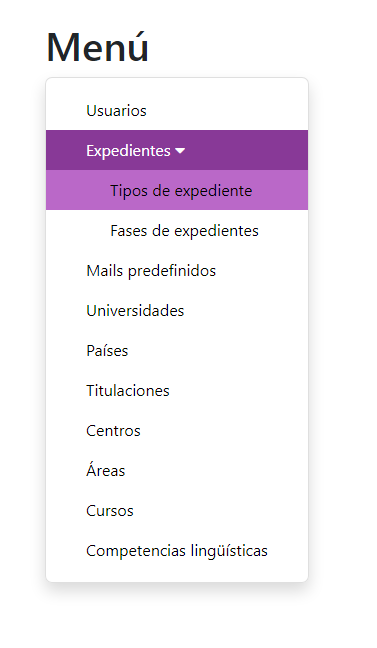
\includegraphics[height=0.4\textheight]{Capturas de twinX/sidebar_panel}
	\caption{Menú lateral del panel en twinX}
	\label{fig:sidebarpaneltwinX}
\end{figure}

Para conseguir el funcionamiento de \textit{dropdown}, hemos escrito el siguiente código con jQuery (\texttt{backend/web/js/dropdown\_expediente\_panel.js}):

\begin{minted}[frame=lines]{javascript}
	let submenusExpedientes = ['tipo-expediente', 'fase-expediente', 'envio-mail-fase'];
	$(document).ready(function() {
		submenusExpedientes.forEach(function (str) {
			if (window.location.pathname.includes(str))
			toggleCollapse();
		});
	});
\end{minted}

El resultado es el menú de la figura \ref{fig:usuariostwinX}. Normalmente, las tablas CRUD suelen tener un botón verde que permiten crear un nuevo registro, pero en el caso de los usuarios, se ha eliminado, ya que al crearlo manualmente desde este menú, no se genera un hash para la contraseña, al mismo tiempo que tampoco tiene gran relevancia el poder crear usuarios desde el panel de control, cuando el principal interés está puesto en gestionar los permisos de los integrantes de la comunidad.

\begin{figure}
	\centering
	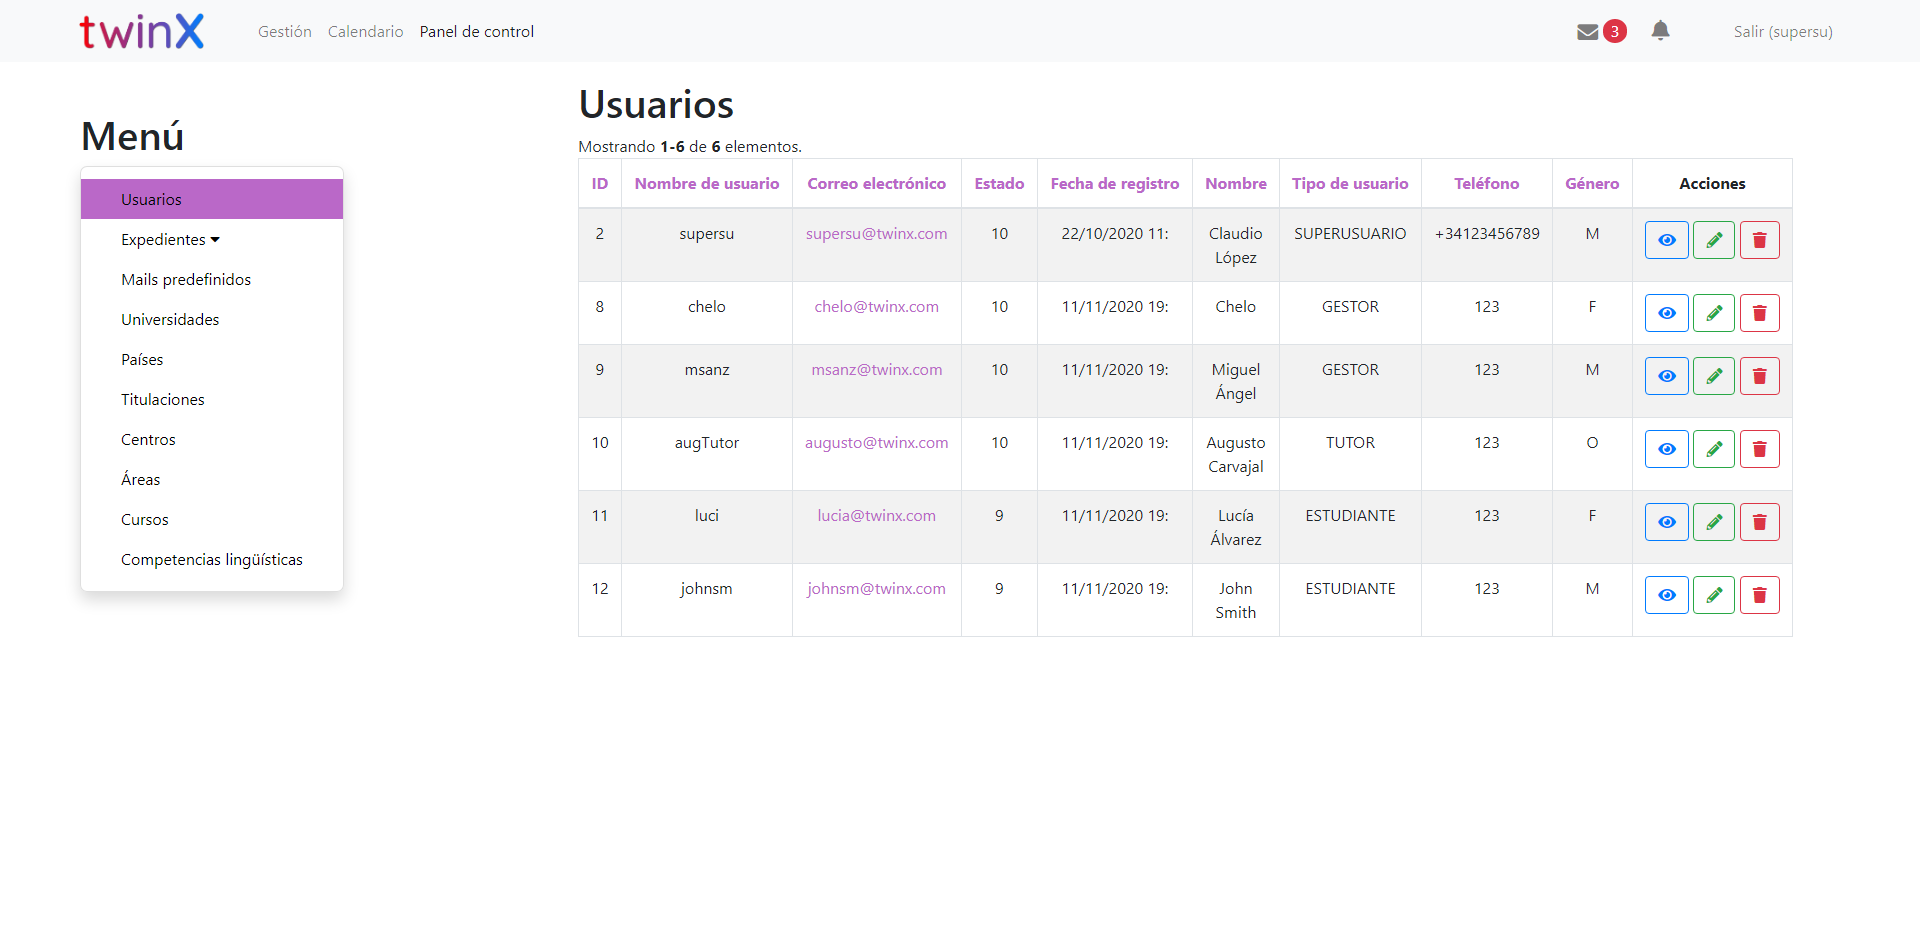
\includegraphics[width=\textwidth]{Capturas de twinX/usuarios_twinX}
	\caption{Menú de usuarios en twinX}
	\label{fig:usuariostwinX}
\end{figure}

Como ya hemos señalado con anterioridad, se tomó la decisión de mantener las vistas de los registros almacenados sin apenas modificar en este módulo de panel de control. Por defecto, lo que podemos ver en la interfaz de vista de un registro es lo que encontramos en la figura \ref{fig:vistatitulaciontwinX}.

\begin{figure}
	\centering
	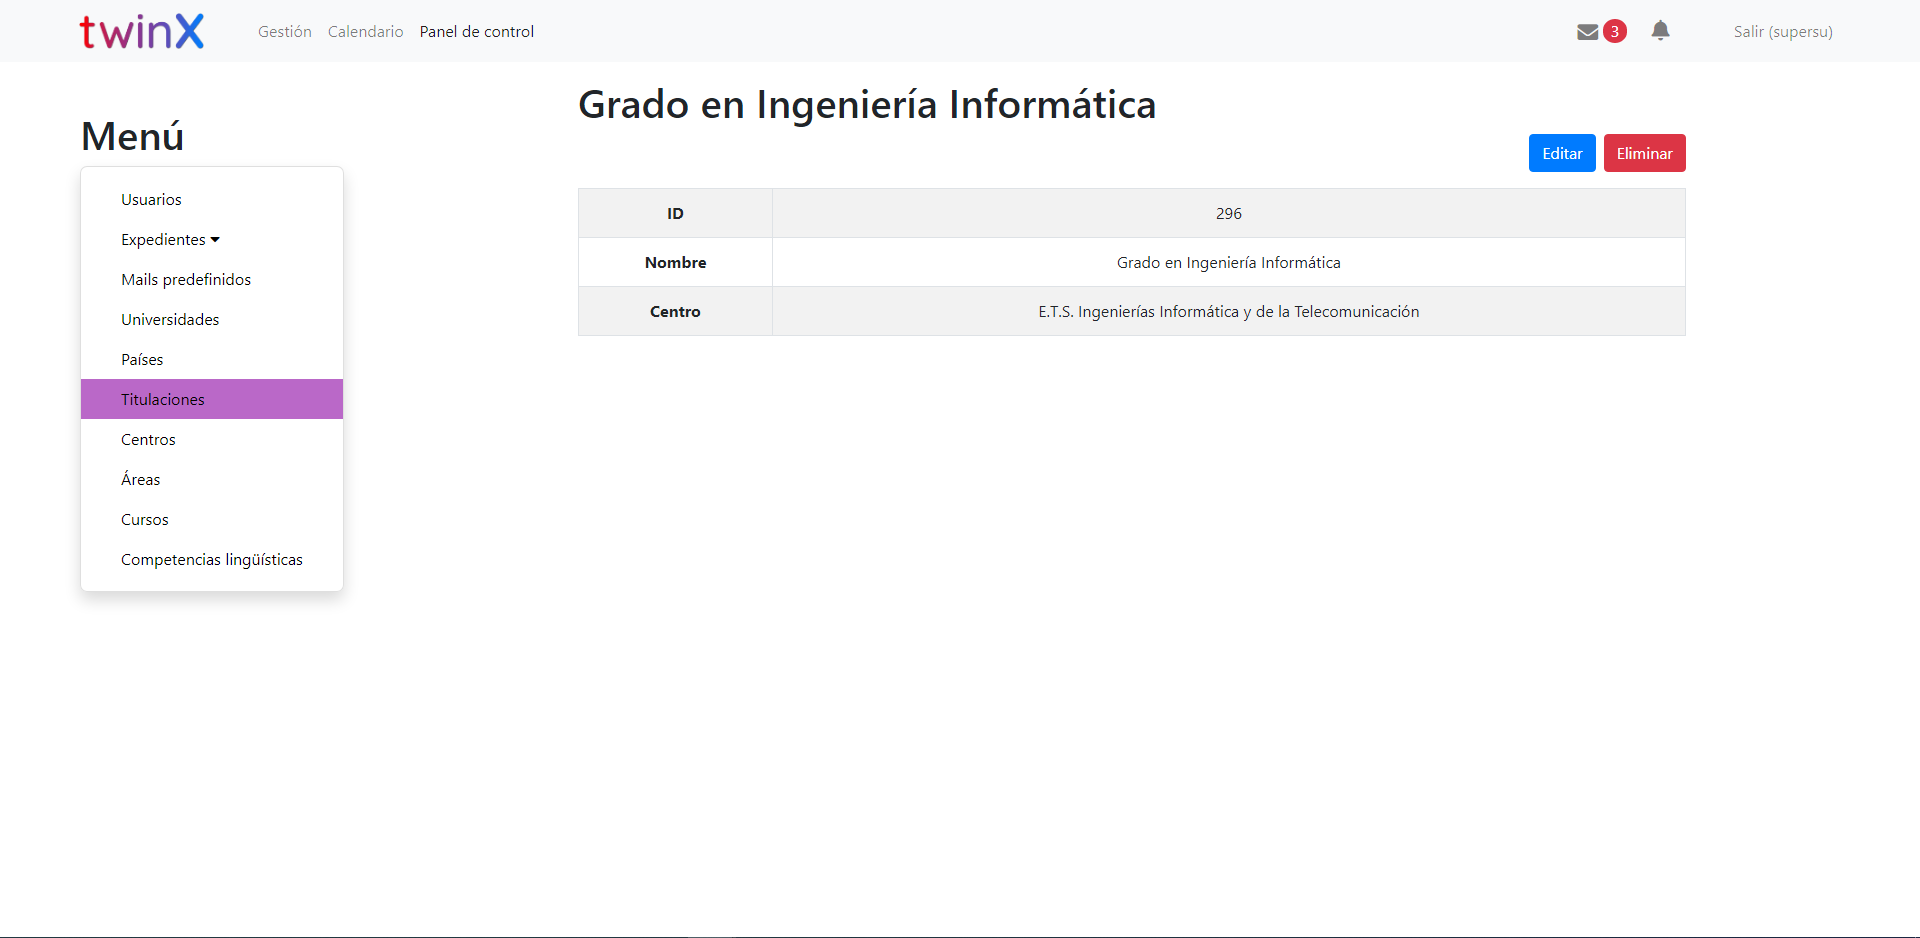
\includegraphics[width=\textwidth]{Capturas de twinX/vista_titulacion}
	\caption[Vista de un registro en twinX]{Vista de un registro en twinX (menú de titulaciones)}
	\label{fig:vistatitulaciontwinX}
\end{figure}

Por defecto, Gii pone los botones justo a la izquierda de las cabeceras de las tablas y de las vistas. Sin embargo, hemos tomado la decisión de modificar esto, como se puede apreciar en la figura \ref{fig:vistatitulaciontwinX}, donde los botones de «editar» y «eliminar» están a la derecha. El motivo es porque mayormente en las tablas del menú \texttt{index} de cada categoría, como la de la figura \ref{fig:fasesexpedientesindex} se podía ver un exceso de información de haber dejado el botón en la izquierda, pues tendríamos el título, el indicador del total de elementos de la tabla y el botón. Por tanto, hemos dejado todos los botones a la izquierda en las sucesivas vistas de los menús de toda la plataforma. Por supuesto, no hemos hecho los cambios de forma manual, sino que se ha modificado el código del generador de Gii para que todas las genere automáticamente como describimos. Esto es posible modificando el archivo \texttt{index.php} para la tabla del menú y el \texttt{view.php} para la vista de un registro en el directorio \texttt{vendor/yiisoft/yii2-gii/src/generators/crud/default/views}\footnote{Este directorio no se encuentra en el respositorio de GitHub \cite{repogit}, dado que forma parte de los archivos del motor de Yii y se encuentran dentro del archivo \texttt{.gitignore}, por lo que no se guardan, dado que pueden obtenerse clonando el repositorio de Yii \cite{yii2advanced}}.

\begin{figure}
	\centering
	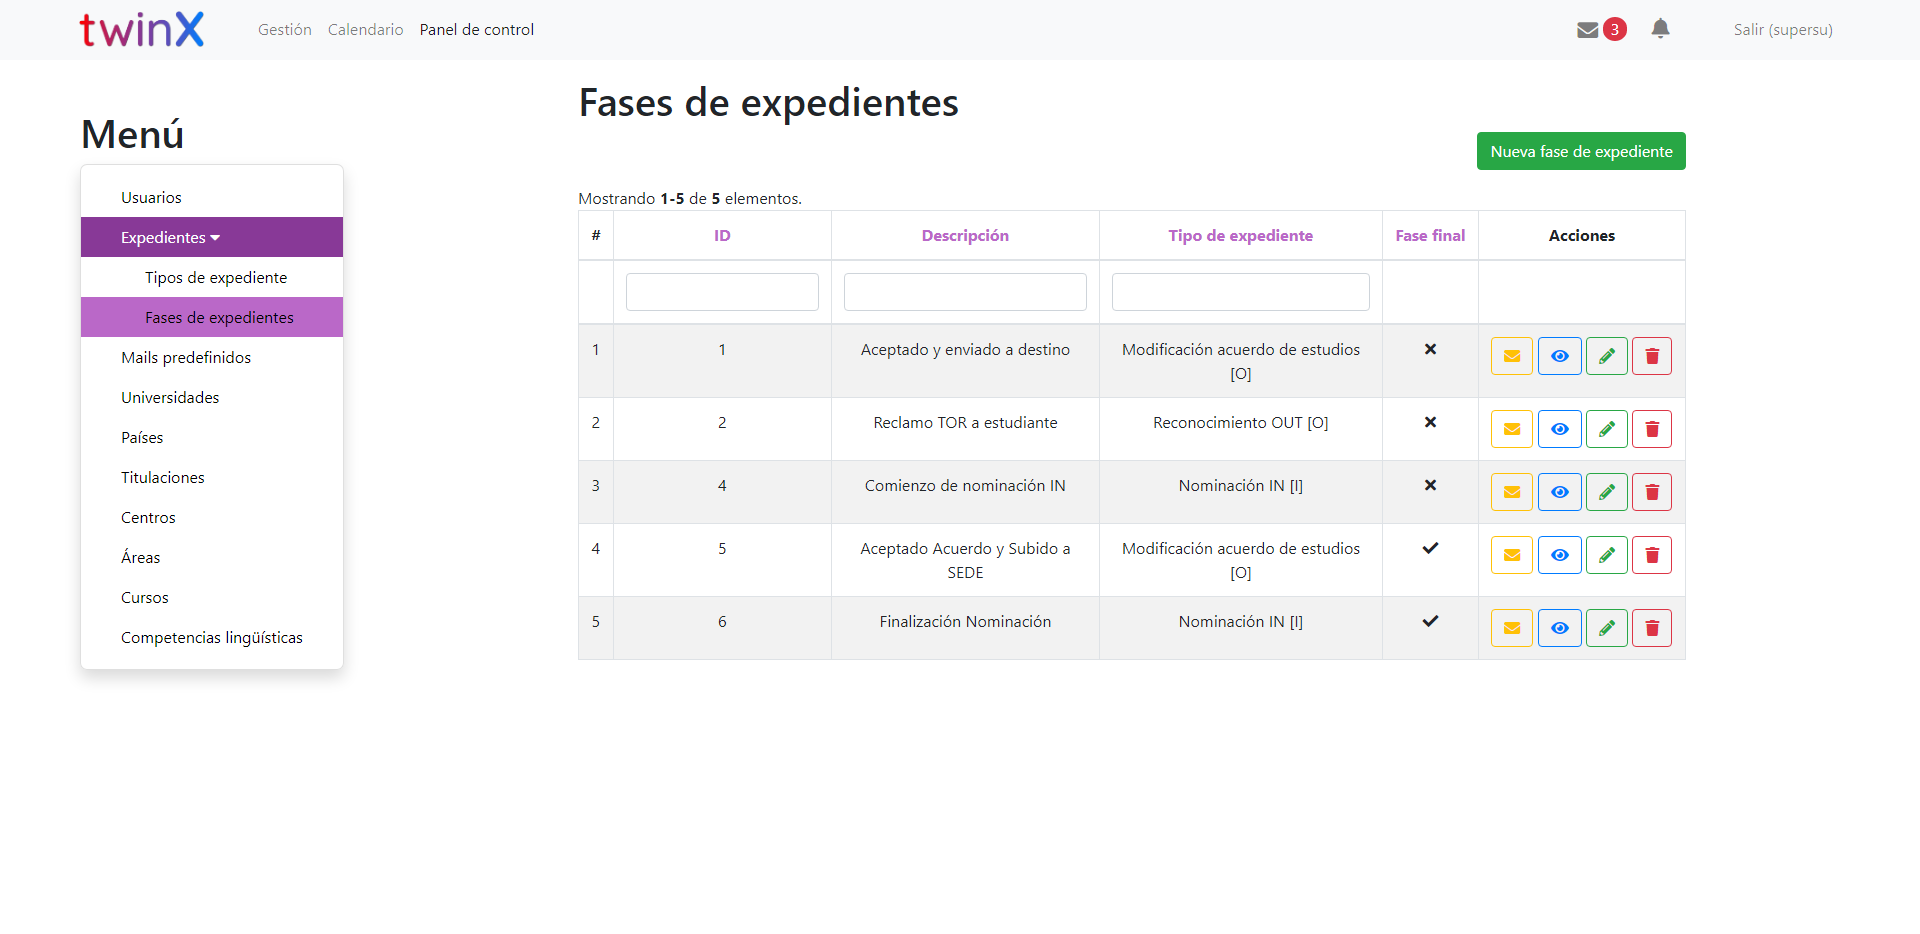
\includegraphics[width=\textwidth]{Capturas de twinX/fases_expedientes_index}
	\caption{Menú de fases de expedientes en twinX}
	\label{fig:fasesexpedientesindex}
\end{figure}

Por último, vamos a destacar la vista de una fase de expediente. Recordemos que el procesar una fase implicaba enviar varios correos a responsables y a destinatarios relacionados con la situación del estudiante (o incluso a él mismo). Por tanto, hemos incluido en la vista de las fases, los mensajes que se enviarían tras procesarla (figura \ref{fig:fasesexpedientesvista}). También podemos verlos pulsando en el botón amarillo con el sobre de la figura \ref{fig:fasesexpedientesindex}, donde se dan aún más opciones al usuario. La implementación de esta parte no es compleja pero sí tediosa, por lo que vamos a omitir su explicación por el momento, dado que en la próxima sección veremos otro ejemplo, ya que en el módulo de gestión \ref{sec:gestion} hemos diseñado una vista compuesta de forma similar.

\begin{figure}
	\centering
	\includegraphics[width=\textwidth]{"Capturas de twinX/fases_expedientes_vista"}
	\caption{Vista de una fase de expediente en twinX}
	\label{fig:fasesexpedientesvista}
\end{figure}

\section{Desarrollo del módulo de gestión}



